This paper combines a number of different data sources to estimate the fields in equation \ref{eq:NVI}. What follows is a description of those data sources and any decisions made in how to best utilize them. The resulting datasets yields a quarterly series for the NVI spanning 2002:Q1 to 2016:Q4.

\subsection{Assets and Liabilites of Bank Holding Companies}

Line-item balance sheet information for bank holding companies comes from quarterly filings of the Federal Reserve's FR-Y9C reporting form\footnote{An FR-Y9C filing is required by each domestic bank holding company (BHCs), savings and loan holding company, US intermediate holding company, and securities holding company with total assets exceeding one billion dollars}. The public nature of this data, as well as the level of granularity in reported asset and liability classes, make this form particularly well-suited to our analysis.

Our objective in using FR-Y9C data is to estimate the outside assets and liability connectivity of each firm in the FR-Y9C's sample. This involves classifying each of the form's asset and liability line items as \textit{inside} or \textit{outside} the financial system. We produce this classification for each of the line items in the current FR-Y9C balance sheet, and apply those classifications across each firm in the sample\footnote{The `current' iteration of the form used in this paper is that from December 2016. For brevity, we will continue to refer to this as the `current' form.}. In cases where this binary classification seems inappropriate, we split the value of the field, classifying fifty percent of its magnitude as inside the system and fifty percent as outside the system\footnote{Section \ref{sec:robustness} shows that our estimates are not very sensitive to alternative assumptions about the share of inside and outside assets and liabilities in these more ambiguous categories.}. The final two columns of Tables \ref{tab:assets_y9c} and \ref{tab:liabilities_y9c} provide these classification breakdowns for current variables (or groups of variables) in the form. 

In past versions of the form, line-items were often less granular. To apply our inside-vs-outside classifications (made based on the current form's line-items) backward to previous form versions, we find the variables in each past form that include the same assets or liabilities as a given group of variables in the current form (the latter group of variables is typically larger, reflecting a movement towards. increasing form granularity over time). We then compute a firm-specific percentage of the total value of the current-form variable group that is attributable to each individual variable in the group during the first year that the variable group was reported\footnote{To consider a simple but illustrative example - say we have determined that the asset categories contained in variables Y1 and Y2 of the current form are the same as those in variable X from some earlier version of the form. We then define $P_{Y1,i}$ and $P_{Y2, i}$ for firm i as the average of $\frac{Y1_i}{Y1_i+Y2_i}$ and $\frac{Y2_i}{Y1_i+Y2_i}$ in the first year that both Y1 and Y2 are reported. Firm i's imputed values for Y1 and Y2 in the early sample then becomes $P_{Y1,i}X$ and $P_{Y2, i}X$.}. By applying this estimated share back through time to 2002, we create a series for each FR-Y9C variable that is roughly consistent over time\footnote{In practice, these breakdowns are only important when the group of current-form variables includes two or more different in-vs-out classifications. Otherwise, the total sum of variables is directed into the same categorization, and any variable-by-variable divisions within the total sum become irrelevant.}. For a detailed view of the current-form variable groups identified, and the method used to extend them back to 2002, see Tables \ref{tab:assets_y9c} and \ref{tab:liabilities_y9c}.

\subsection{FDIC-Insured Deposits of BHCs}\label{subsec:Deposits}

We wish to avoid classifying any FDIC-insured deposits from the commercial bank subsidiaries of BHCs as inside the financial system, since those deposits are likely not held by financial firms and are ultimately government liabilities (which reside outside the network). To separate FDIC-insured deposits from a BHC's total deposits, we use quarterly data from the FFIEC 041 (also known as the Call Report), as collected by the Federal Financial Institutions Examination Council\footnote{More specifically, our primary variables of interest from the form are RCON2200 (total domestic deposits) and RCON5597 (estimate of uninsured domestic deposits). Our estimate of insured deposits becomes the difference between these two fields. It is worth noting that our final estimate of uninsured deposits (which is then used in our index) is the difference between this estimate of insured deposits and the FR-Y9C form's value for firm domestic deposits (\textit{not} the Call Report's domestic deposits variable). It is our understanding that the FR-Y9C form, as it pertains to entire BHCs instead of just commercial bank subsidiaries, includes a better estimate of total deposits for our purposes.}. After matching each commercial bank to its BHC parent, we subtract the estimated quantity of FDIC-insured deposits, as reported in the Call Report, from the BHC's total deposits. Only this final ``uninsured'' value of deposits is considered inside the financial system, for the purposes of further analysis\footnote{In our benchmark setup for the NVI, 100\% of uninsured domestic deposits are counted as \textit{inside} the system. While this is likely close to accurate for the custodian banks (banks whose deposits are primarily safeguards of the assets of other banks) in our sample -- namely State Street and Bank of New York Mellon -- this is certainly unrealistic for many of the other BHCs in our panel. Section \ref{sec:robustness} includes robustness exercises on different configurations, including one allowing for more firm-specific allocation percentages. In short, this decision makes little difference in our final NVI series.}.

The process of matching Call Report data to balance sheet data on its BHC parent can become complicated, particularly around BHC mergers, acquisitions, or legal classification changes. To find the final BHC parent of each commercial bank, we use a bank-parent matching hierarchy maintained by the Federal Reserve Bank of New York. We then match commercial banks to their parent BHCs based on the BHC's RSSID identifier code. When this process does not lead to any commercial bank matches for a given BHC, we then match that BHC to all the commercial banks owned by the BHC's parent organization. This can occassionally lead to overestimates of the FDIC-insured deposits of these BHCs, but we have found that this process almost always yields sensible-looking series for these BHCs' financial connectivities. The alternative approach, where we do not conduct the second matching procedure and list FDIC-insured deposits as `0' for these firms, often yields impractically-large financial connectivities.  

\subsection{Probabilities of Default}

The probabilities of default $\delta$ for each firm in equation \ref{eq:NVI} are the true - or physical - probabilities of default. As such, any risk-neutral estimate of a firm's default probability (such as those commonly extracted from credit default swaps or corporate bond spreads) would be inappropriate for calculating our NVI.

We consider Moody's Analytics' (formerly KMV's) Expected Default Frequency (EDF) series to be suitable for our analysis. The EDF measure uses typical lognormal assumptions and an options-pricing approach to equities to determine which variables should theoretically be important for determining a given firm's probability of default. They then use them to fit an empirical model of default probabilities using Moody's extensive database of historical defaults, as explained in \citet{kmv_methods}\footnote{Moody's historical defaults dataset considers government rescues as default events, if the rescue specifically saved the firm from default. So, in that sense, the EDF series can be considered as a probability of default without government intervention. As the model of \citet{glasserman2015likely} does not include the possibility of government rescue, this empirically estimated probability closely matches its model counterpart.}.

Equation \ref{eq:NVI} calls for the probability of default due to shocks to outside assets, although Moody's Analytics' EDF makes no distinction between the actual sources of default losses. Rather than attempt to back out the theoretically-appropriate default probability from these EDFs, we simply include the EDF value itself as $\delta_i$ for each firm in equation \ref{eq:NVI}, with the understanding that this probability is in fact an upper-bound on the direct default probability. Relying on the fact that the NVI is itself an upper-bound, the bounds obtained from an NVI calculated this way will still be valid. 

Moody's EDF model produces a daily series of physical expected default frequencies at one-year horizons. We define a firm's quarterly EDF measure to be the average of its daily measures over a given quarter.

\subsection{Non-BHC Financial Firms} \label{subsec:non_bhc}

For financial firm subsectors whose firms do not file FR-Y9C forms, we include nodes into the NVI using less granular firm-level balance sheet information and subsector-level data on assets and liabilities from the Financial Accounts of the United States, maintained by the Board of Governors of the Federal Reserve System.

To incorporate a new firm (or, in this case, group of firms) into our NVI measure requires us to know each firm's individual default probability $\delta_i$, its outside assets $c_i$, and that firm's liability connectivity $\beta$ \textit{if} that firm's $\beta$ becomes the new $\beta^+$ for the system. We first make the necessary simplifying assumption that the $\beta^+$ selected from the firms in our FR-Y9C sample correctly identifies the $\beta^+$ for the entire network\footnote{In fact, the $\beta^+$ we select from the FR-Y9C sample for the NVI is the highest financial connectivity found in the top 20 BHCs by assets. See \ref{sec:robustness} for a discussion of this decision, and an analysis of robustness to different selections.}.

Left to determine is how the inclusion of other financial subsectors affects the other component of the NVI, the weighted average default probability $\frac{\sum {\delta _{i}c_{i}}}{\sum {c_{i}}}$. We approximate the value of this componenet for the subsectors not covered by the FR-Y9C by first constructing an estimate of the total outside assets of each of those subsectors from the Financial Accounts of the United States and then computing an average default probability weighted by assets for each new subsector using total firm asset values and Moody's EDF measures. Total quarterly assets for each firm, compiled from that firm's financial releases and filings, are also available in the Moody's EDF dataset\footnote{This is done using a method similar to that for the FR-Y9C, categorizing different Financial Accounts asset classes as inside or outside the system. See Table \ref{tab:ffunds_inout} for the precise `inside' vs `outside' classification used for different variables in the release. Line-items from the Financial Accounts are much coarser than those in the FR-Y9C, making this an admittedly cruder method of classification. As Section \ref{sec:robustness} shows, however, this breakdown has very little effect on the final NVI measure.}.

More explicitly, let $Y$ denote the set of firms in our FR-Y9C sample, $S = \{S_1, S_2, \cdots\}$ denote a set of sets, with each individual element $S_j$ being the set of firms belonging to some new financial subsector, and let $A$ denote the entire financial network $Y \cup S$. Then, 
\begin{equation}\label{eq:approx}
\frac{\Sigma_{A} \delta_i c_i}{\Sigma_A c_i} = \frac{\Sigma_Y \delta_i c_i+ \Sigma_{S_j \in S}(\Sigma_{i \in S_j } \delta_ic_i)}{{\Sigma_Y c_i}  + \Sigma_{S_j \in S}(\Sigma_{i \in S_j}c_i)} \approx \frac{\Sigma_Y \delta_i c_i+ \Sigma_{S_j \in S}(\bar{\delta_{S_j}}\Sigma_{i \in S_j} c_i)}{{\Sigma_Y c_i} + \Sigma_{S_j \in S}(\Sigma_{i \in S_j}c_i)} 
\end{equation}
\begin{equation}
\text{where } \bar{\delta_{S_j}} = \frac{\Sigma_{i \in S_j} \delta_i a_i}{\Sigma_{i \in S_j}a_i}, \text{with } a = \text{total assets of firm i} \label{eq:avg_def}
\end{equation}
This computation is only an approximation of the true $\frac{\Sigma_{A} \delta_i c_i}{\Sigma_A c_i}$ for two reasons. First, the weighted average probability of default per sector $\bar{\delta_{S_j}}$ is weighted here by \textit{total assets} per firm, where a more precise measure for the NVI would be weighted by \textit{outside assets} per firm. Second, and more significantly, our sample of average default probability is limited to those firms for which we have a Moody's EDF measure - namely, to publicly-traded firms. Provided that our computed averages are good representations of the entire sector, then the NVI constructed using this approximation should remain a useful upper-bound on network spillovers that allows us to include a much larger portion of the US financial system than the FR-Y9C sample alone would allow.

\subsection{Subsector EDF Samples}

Per Section \ref{subsec:non_bhc}, we wish to include subsector-wide averages in our NVI for security broker dealers, insurance companies, real estate investment trusts, and an `other' category for several other types of financial firms. To determine which firms should comprise each subsector's sample in equation \ref{eq:avg_def}, we use Moody's Analytics' own internal sectoral classification system, pairing their categorizations with the subsector definitions given in the Financial Accounts of the United States. For the purposes of calculating outside assets $c$ for the `other' sector, we sum across the Financial Accounts subsectors for credit unions, finance companies, funding corporations, and issuers of asset-backed securities\footnote{The `other' category is the only one for which finding an appropriate subsample within the EDF dataset it not straightforward. We choose to include any firms with sectoral tags of `Finance Companies', `Investment Management', or `Finance Not Elsewhere Classified' in this node's average probability calculation.}.

To show the relative magnitude of assets assigned to these difference subsectors by the Financial Accounts of the United States, we plot the percentage of total network assets (defined as the sum of total financial assets in each subsector described above, plus the Financial Accounts' total financial assets for BHCs) attributable to each of these subsectors in Figure \ref{fig:ffunds_assets}. As Figure \ref{fig:ffunds_assets} shows, BHCs are by far the largest financial subsector by assets, meaning that the weights given to BHCs' default probabilitys will, in aggregate, be larger than the weights assigned to any of the included subsectors.  

\begin{figure}
\begin{center}
\includegraphics[width = \textwidth]{../output/ffunds_assets_area.pdf}
\end{center}
\caption[]{\textbf{Total Financial Assets for each Network Subsector, as a Percentage of Total Network Assets.} According to the Financial Accounts of the United States, BHCs comprise by far the largest percentage of network assets}\label{fig:ffunds_assets}
\end{figure}

%\begin{figure}
%\begin{center}
%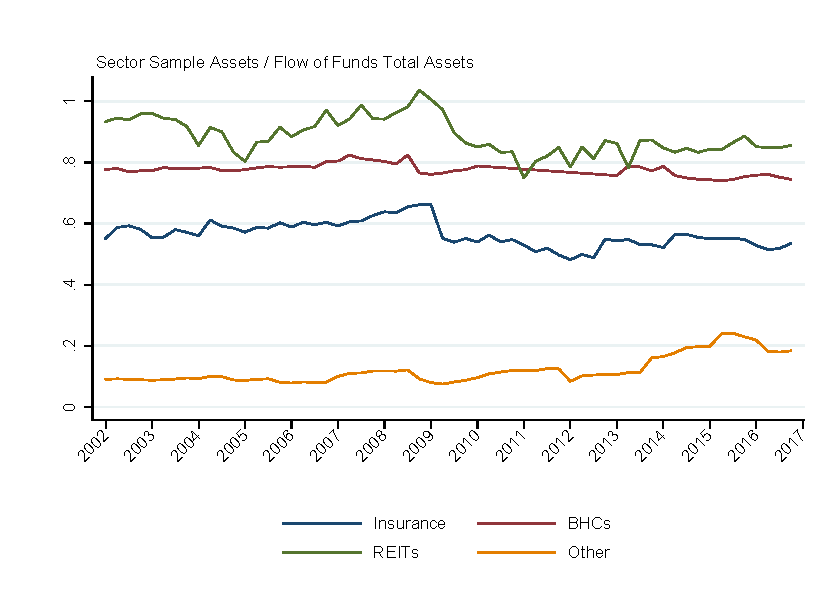
\includegraphics[width = \textwidth]{../output/coverage.pdf}
%end{center}
%\caption[]{\textbf{Data Coverage of Compustat Subsample.} Only a subsample of firms in each subsector are available to calculate a sector-wide probability of default, which is then used to approximate our network vulnerability measure for a network including these subsectors. The percent of sector assets covered for insurance companies and bank holding companies is relatively high and stable. Data coverage for broker-dealers is very high before the financial crisis, then drops. Real estate investment trusts are well-covered by the EDF dataset, while the umbrella category of `other' is not.}\label{fig:coverage}
%\end{figure}

\begin{figure}
\begin{center}
\includegraphics[width = \textwidth]{../output/coverage_broad.pdf}
\end{center}
\caption[]{\textbf{Data Coverage of EDF Sample for NVI, Against Total Network Assets.} Only a subsample of firms in each subsector have their default probabilities directly enter the NVI. The first line sums the total assets of firms whose EDF measures enter the NVI in some form - either individually if that firm filed an FR-Y9C, or as part of a subsector average default probability sample - divided by total network assets from the Financial Accounts of the United States. The second line plots the same, if we instead consider each approximated subsector node per equation \ref{eq:approx} to cover the entire sum of that subsector's assets.}\label{fig:coverage_broad}
\end{figure}

To assess whether the samples used to compute each of the default probabilities within equation \ref{eq:approx}, in Figure \ref{fig:coverage_broad} we plot the percentage of total network assets (with the `network' defined as the sum of total financial assets in the subsectors of Figure \ref{fig:ffunds_assets}) that are accounted for by the total assets of firms whose default probabilities directly enter into the NVI - either individually if that firm files an FR-Y9C, or as part of the sample for computed a subsector's average default probability. The red line in Figure \ref{fig:coverage_broad} plots the same value, if we consider each approximated node in equation \ref{eq:approx} to cover all of the assets from that subsector's Financial Accounts entries. The blue line shows that even the most conservative measure covers consistently more than 50\% of the assets of the entire U.S. financial system. If we consider our network to cover the sectors of each approximated subsector node, that coverage becomes even higher, as shown in the red line of Figure \ref{fig:coverage_broad}\footnote{Note that the actual assets attributed to each subsector for the purposes of calculating these coverage statistics are total subsector assets \text{after} any deductions from FR-Y9C sample overlap. This adjustment, as well as the fact that FR-Y9C coverage of BHC assets in the Financial Accounts is not 100\%, are why the second line in Figure \ref{fig:coverage_broad} is not mechanically 100\%.}.


%$\bar{\delta_{S_j}}$ cover a reasonably-wide array of each subsector's assets, we plot the share of total sector assets (computed from the Financial Accounts of the United States) that are accounted for by the subsample of firms used to calculate the average sector default probabilities. The results of this exercise are presented in Figure \ref{fig:coverage}\footnote{See \ref{sec:appendixb} for a discussion of why coverage for broker dealers is low, and why we do not believe this is cause for major concern in our estimate.}.

%The coverages of our insurance company subsample and our Y9C sample (the denominator for which is the sum of total assets in `private depository institutions' and `holding companies' from the Flow of Funds) are both relatively high and reasonably stable over our sample period. The coverage for security brokers and dealers is very high before the financial crisis, but then drops precipitously. To understand why this occurs, and why we do not believe it is cause for concern, we also show \Cref{fig:dealer_coverage_details}, which compares the timing of that drop with several large-scale acquisitions and firm classification changes around that time. The drops in dealer coverage exactly coincide with acquisitions of broker dealer firms by BHCs included in our FR-Y9C sample, as evidenced by the spikes in assets of JP Morgan and Bank of America at the same times as coverage drops. Low coverage is further exacerbated by the inclusion of Goldman Sachs and Morgan Stanley in the FR-Y9C sample at the same time. When a firm is included in the FR-Y9C sample, it is \textit{excluded} from the subsample of sector firms used to calculate that sector's average probability of default (and its assets are also excluded from that sector's estimate of total outside assets, also used in the NVI). Thus, the low `coverage' of broker-dealers later in the sample is not a result of assets being excluded from the sample - but rather a shift in categorization of certains firms from subsamples $B$ to $Y$, to use the nomenclature above.


\subsection{Defaulting firms}

The model of \citet{glasserman2015likely} includes an explicit assumption that no nodes included in the system are initially in default (defined as having book liabilities greater than book assets). To avoid including any such firms in our estimates of equation \ref{eq:approx}, we use Moody's Analytics' Default and Recovery Database to identify dates of bankruptcy filing. If a firm files for bankruptcy at any point during our sample period (2002-Q1 to 2016-Q4), then no expected default frequency data is used for that firm after the date of filing.